%%% Template originaly created by Karol Kozioł (mail@karol-koziol.net) and modified for ShareLaTeX use

\documentclass[a4paper,11pt]{article}
\usepackage{float}
\usepackage[T1]{fontenc}
\usepackage[utf8]{inputenc}
\usepackage{graphicx}
\usepackage{xcolor}

\renewcommand\familydefault{\sfdefault}
\usepackage{tgheros}
\usepackage[defaultmono]{droidmono}

\usepackage{amsmath,amssymb,amsthm,textcomp}
\usepackage{enumerate}
\usepackage{multicol}
\usepackage{tikz}
% subfigures
\usepackage{caption}
\usepackage{subcaption}

\usepackage{geometry}
\geometry{total={210mm,297mm},
left=25mm,right=25mm,%
bindingoffset=0mm, top=20mm,bottom=20mm}

\usepackage[
backend=biber,
style=alphabetic,
sorting=ynt
]{biblatex}

\addbibresource{bibliography.bib} % imports bibliography file


\linespread{1.3}

\newcommand{\linia}{\rule{\linewidth}{0.5pt}}

% custom theorems if needed
\newtheoremstyle{mytheor}
    {1ex}{1ex}{\normalfont}{0pt}{\scshape}{.}{1ex}
    {{\thmname{#1 }}{\thmnumber{#2}}{\thmnote{ (#3)}}}

\theoremstyle{mytheor}
\newtheorem{defi}{Definition}

% my own titles
\makeatletter
\renewcommand{\maketitle}{
\begin{center}
\vspace{2ex}
{\huge \textsc{\@title}}
\vspace{1ex}
\\
\linia\\
\@author \hfill \@date
\vspace{4ex}
\end{center}
}
\makeatother
%%%

% custom footers and headers
\usepackage{fancyhdr}
\pagestyle{fancy}
\lhead{}
\chead{}
\rhead{}
\lfoot{Assignment \textnumero{} 5}
\cfoot{}
\rfoot{Page \thepage}
\renewcommand{\headrulewidth}{0pt}
\renewcommand{\footrulewidth}{0pt}
%

% code listing settings
\usepackage{listings}
\lstset{
    language=Python,
    basicstyle=\ttfamily\small,
    aboveskip={1.0\baselineskip},
    belowskip={1.0\baselineskip},
    columns=fixed,
    extendedchars=true,
    breaklines=true,
    tabsize=4,
    prebreak=\raisebox{0ex}[0ex][0ex]{\ensuremath{\hookleftarrow}},
    frame=lines,
    showtabs=false,
    showspaces=false,
    showstringspaces=false,
    keywordstyle=\color[rgb]{0.627,0.126,0.941},
    commentstyle=\color[rgb]{0.133,0.545,0.133},
    stringstyle=\color[rgb]{01,0,0},
    numbers=left,
    numberstyle=\small,
    stepnumber=1,
    numbersep=10pt,
    captionpos=t,
    escapeinside={\%*}{*)}
}

%%%----------%%%----------%%%----------%%%----------%%%

\begin{document}

\title{Reinforcement Learning Assignment \textnumero{} 2}

\author{Ruslan Burakov, s1569105}

\date{17/03/2015}

\maketitle
\section*{Note} 
All full code fragments are located in the end of the report in the appendix section.
Naming convention. By one episode I mean period when agent is initialised randomly within maze and it tries to reach goal. So learning process consists of many episodes. Once the learning is over and the final policy is evaluated I call it the end of experiment. I repeat several experiments to determine mean convergence time and confidence intervals.

% \begin{figure*}[htbp!]
%     \centering
%     \begin{subfigure}[t]{0.75\textwidth}
%         \centering
%         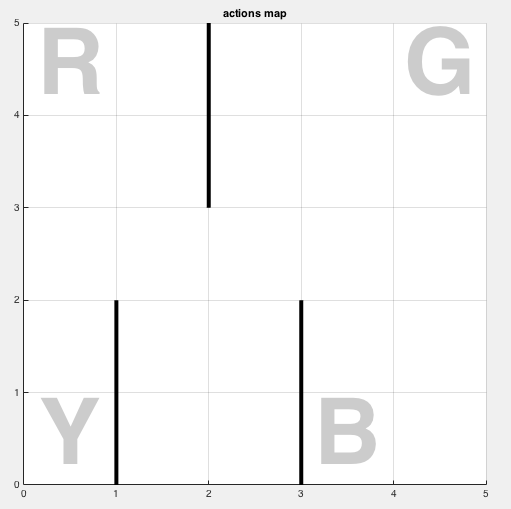
\includegraphics[height=3in]{maze}
%     \end{subfigure}%
%     \caption{Taxi problem maze}
%     \label{fig:taxi_maze}
% \end{figure*}
% \subsection{Typical time horizon of the problem}

\section{Function Approximation Discussion}
According to the lectures Q function can be approximated by k basis function in the following expression:
\begin{align}
    \label{eq:approxQ}
    Q(s,a) = w_1 f_{1}(s,a) + w_2 f_{2}(s,a) + \ldots + w_k f_{k}(s,a) = w^{T} f(s, a)
    \\
    \text{ s - state, a - action}
\end{align}

For this question and following ones our basis functions can be partitioned into this product:
\begin{equation}
    f_{i}(s, a) = f_{i}(s) f_{i}(a)
\end{equation}
In the expression above each i'th basis function which depends only on action is  \[ f_{i}(a) = I(a=a')\] where $I(a=a')$ is identity/indicator function of particular action. In the assignment we use 25 basis functions which depends only on the state $f_{i}(s)$ and also we have 5 different actions which means we need 5 action basis functions $I(a=a')$ and therefore by multiplying these domains we will get the following number of general basis functions:
\begin{equation}
|f_{i}(s, a)| = |f_{i}(s)| * |f_{i}(a)| = 25 * 5 = 125
\end{equation}
and due to this we get that in \ref{eq:approxQ} we have 125 weights overall or 25 weight per 5 actions. This can be simplified even further during the learning step (here I omit indexes which means that these are vectors):
\begin{align}
\delta \leftarrow r + \gamma max_{a' \in A} w^{T} f(s', a') - w^{T} f(s, a) \\
w \leftarrow w + \eta \delta f(s, a) \\
\end{align}
by using the fact that $f_{i}(a) = I(a=a')$ and noting that all actions which differs from action identity will make no contribution in the product $w^{T} f(s, a)$: 
\begin{align}
    \label{eq:simpleApprox}
Q(s,a) = w1_a f_{1}(s) + w2_a f_{2}(s) + \ldots + w25_a f_{25}(s) = w^{T}_{a} f(s) \\
\delta \leftarrow r + \gamma max_{a' \in A} w^{T}_{a'} f(s') - w^{T}_{a} f(s) \\
w_a \leftarrow w_a + \eta \delta f(s) \\
\text{where each $w_a$ is 25 vector of weights which corresponds to particular action $a$}
\end{align}

Relying on the fact that our task is discrete one I precompute values of each 25 basis functions for each cell of maze in order to save computational time. Here how it looks approximately in my code (particular cases for identity functions $f_{i}(s)=I(s=s_i)$ or RBF are in the appendix) like this:
\begin{lstlisting}[language=Octave]
  %...
  %precompute basis functions in advance
  % number of states
  Sx = 10;  % width of grid world
  Sy = 10;  % length of grid world
  M = 2; % cover neighbouring area
  %basis functions
  F = zeros(Sx, Sy, 25);
  
  %iterate through maze cells
  for ix = 1:Sx
    for iy = 1:Sy
      %identity functions
      %iterate through 25 basis functions
      for kx = 1:5
        for ky = 1:5
          %basis function index (can be from 1 to 25)
          fId = 5 * (ky - 1) + kx;
          %Here it is identity functions 
          %It can be RBF as well
          F(ix, iy, fId) = M*(kx-1) < ix && ix <= M*kx &&...
                           M*(ky-1) < iy && iy <= M*ky;
        end
      end
    end
  end
  
  %EPISODES/LEARNING LOOP GOES BELOW
  %...
\end{lstlisting}
These give sufficient speed up, especially when using RBF (almost 20 times). Also, in terms of computation speed there is basically no difference whether identity functions or RBF are used as their precomputed before hand.

Additionally by analysing equations \ref{eq:simpleApprox} it can be seen that it is possible to rewrite them as dot products between vectors and matrices. Code snippet which demonstrates dot products speed ups:
\begin{lstlisting}[language=Octave]
    %...

    %INITIALISATION 
    %number of actions
    A = 5;
    %weights matrix. For each actions keeps values of 25 basis functions
    W = zeros(A,25);
    %basis functions
    F = zeros(Sx, Sy, 25);
  
    %...
    
    %INSIDE PARTICULAR EPISODE
    
    %...
    
    % choosing best action is the dot product
    [V_s0, a0]=max(W * reshape(F(x0, y0, :), 25, 1));  
    
    %...
    
    %learning
    V_s1 = max(W * reshape(F(x1, y1, :), 25, 1)); 
    %approximate Q(s0, a0) by dot product
    Q_s0_a0 = W(a0, :) * reshape(F(x0, y0, :), 25, 1);
    delta = r+gamma*V_s1 - Q_s0_a0;
    %basic functions in state x0 y0
    bfs = reshape(F(x0, y0, :), 1, 25);
    %updating weights matrix
    W(a0, :) = W(a0, :) + eta * delta * bfs;
    
    %...
\end{lstlisting}

Dot products work much faster in contrast to usual for loops in MATLAB. That is why due to such implementation I am able to go trough 150000 episodes with RBF functions on 25 by 25 maze in 2 minutes. 








%------------------ QUESTION 1 END ------------------------------








\section{Identity functions representation in 5x5 maze}
In this task we are using $f_{i}(s)=I(s=s_i)$ as state basis functions.
First of all, let's see results achieved by true Q function (table representation) for this task.
I have used the following learning parameters:
\begin{center}
	\begin{tabular}{| c | c | }
		\hline
		Learning rate $\eta$ &  0.2 \\ 
		\hline
		Exploration rate $\epsilon$ & 0.1 \\ 
		\hline
		Discount rate $\gamma$ & 0.9; \\
		\hline
	\end{tabular}
\end{center}

\begin{figure}[htbp!]
 \centering
 \begin{subfigure}[t]{0.49\textwidth}
 	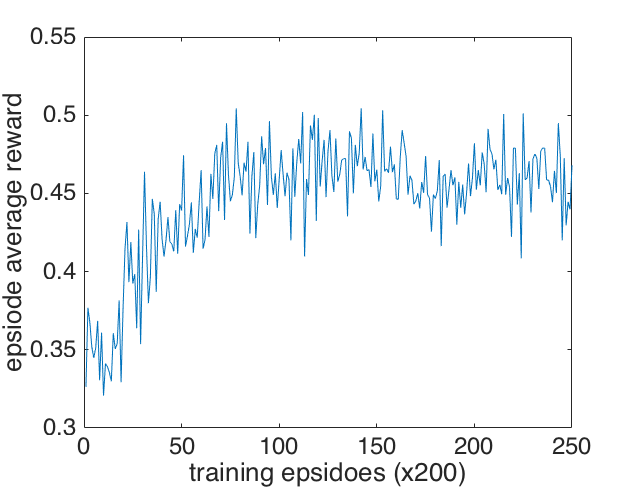
\includegraphics[width=\linewidth]{img/avg_r_true5x5}
 	\caption{Average reward}
 	\label{fig:avg_r_true5x5}
 \end{subfigure}
 ~
 \centering
 \begin{subfigure}[t]{0.49\textwidth}
 	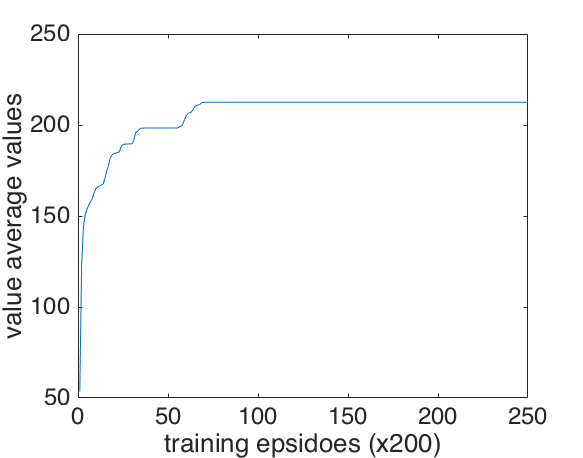
\includegraphics[width=\linewidth]{img/v_true5x5}
 	\caption{Value function convergence}
 	\label{fig:v_true5x5}
 \end{subfigure}
 \\
 \centering
 \begin{subfigure}[t]{0.49\textwidth}
 	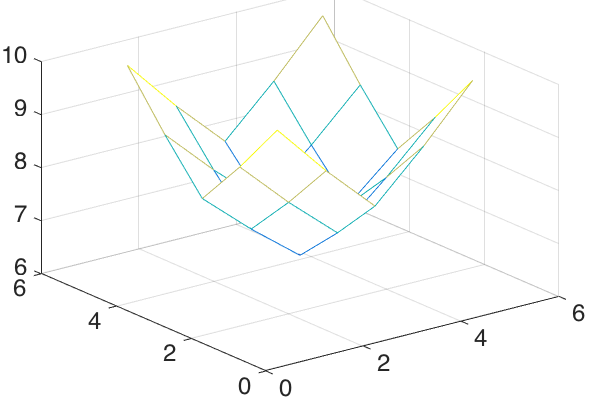
\includegraphics[width=\linewidth]{img/v3d_true5x5}
 	\caption{Final value function on maze states}
 	\label{fig:v3d_true5x5}
 \end{subfigure} 
 ~
 \centering
 \begin{subfigure}[t]{0.49\textwidth}
 	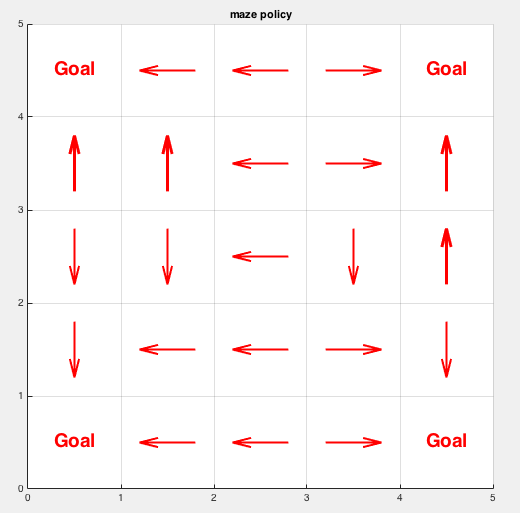
\includegraphics[width=\linewidth]{img/policy_true5x5}
 	\caption{Final policy}
 	\label{fig:policy_true5x5}
 \end{subfigure} 	
 \caption{5x5 maze. Table representation}
 \label{fig:true5x5}
\end{figure}


In this problem our reward doesn't depend on how many steps agent did within one episode in order to reach reward (it is just 1 if agent has reached its goal). That is why reward in the end of one episode is not very representative value in terms of how well the learning process goes as it won't show how fast we reached our goal. Due to that I use average reward per episode, as the more time agent spent in the maze the smaller his average reward will be.

\begin{lstlisting}[language=Octave]
    %...
    %start episode
    for u = 1:Sx*Sy
        %learning and acting in maze
        %...
    
        % goto next episode once the goal is reached
        if ismember([x0, y0], Goals, 'rows') 
          avg_r = r/u;
          %display(avg_r, 'reached the goal!');
          break; 
        end
    end
    %end of episode
    
    %store average reward
    avg_rs(t) = avg_r;
    %...
\end{lstlisting}

All values below are averaged over 200 training episodes () to ease fluctuations due to random starting position and $\epsilon$-greedy learning.

The average reward is presented on Figure \ref{fig:avg_r_true5x5}. It reaches approximately 0.45 which corresponds to the $1/0.45=2.222$ steps in the one episode on average. This is logical as in 5x5 maze with goals in the corners of the maze the average number of steps to reach goal should be between 2 and 3. 

To determine dynamic of learning process more precisely I use value function $V(sx, sy)$. I sum up all entries of value function which corresponds to particular positions in the maze  (we shouldn't have negatives ones because there are no rewards -> only 1 and 0) and rely on the fact that if entries of value function doesn't change then their sum doesn't change, as well. The situations when some entries declined by exactly the same amount other entries increased are extremely unlikely. 
Code snippet which is responsible for this:
\begin{lstlisting}[language=Octave]
  %...    
  % after each episode:
  
  %compute value function 
  VV = max(Q,[],3);%Size: (Sx,Sy)
  %storing for future plotting
  samples(t) = sum(reshape(VV, 1,numel(VV)));
  
  %...
  
  %after end of training
  %averaging to remove most fluctuations
  average_over = 200;
  avg_samples = mean(reshape(samples, average_over, []));
  
  %...
\end{lstlisting}

On Figure \ref{fig:v_true5x5} we can see that values are almost not changed after approximately $160 * 200 = 32000$ episodes. I determine convergence by computing standard deviation of the averaged value function (over 200 episodes) with window 50 and after that I find the first spike in its values from the end. Such procedure allows to avoid determining convergence too early when value function reaches local maximum (on Figure \ref{fig:v_true5x5} the local maximum is reached near $80 * 200 = 8000$). The disadvantage of this method that it doesn't allow to determine convergence online during learning that is why it is impossible to abort learning earlier. 
Code snippet responsible for this:
\begin{lstlisting}[language=Octave]
    %...
    
    %computing standard deviations over window 50
    smp_stds = zeros(1,(size(avg_samples, 2) - 50));
    for t=1:(size(avg_samples, 2) - 50)
      smp_std = std(avg_samples(t:(t+50)));
      smp_stds(t) = smp_std;%abs(avg_samples(t) - avg_samples(t-1))/avg_samples(t);
    end
    
    %find first spike bigger than 0.2 from the end
    convg = find(smp_stds > 0.2, 1, 'last')
    %convergence time
    convg_t = convg * average_over
    %if it is not empty then store in experiment array
    %to compute confidence intervals
    if ~isempty(convg_t)
      convg_times = [convg_times, convg_t];
    end
    
    %...
\end{lstlisting}

Here, I set criteria for standard deviation to be bigger than 0.2 starting from the end in order to determine convergence. 

After repeating experiment for 10 time I got the following results for convergence with $95\%$ confidence interval:

\begin{center}
	\begin{tabular}{| c | c | }
		\hline
		Convergence criteria &  0.2 \\ 
		\hline
		Number of experiments & 10 \\ 
		\hline
	    Mean convergence time & 15480 $\pm$ 2462 episodes \\
		\hline
	\end{tabular}
\end{center}

Finally, on Figure \ref{fig:v3d_true5x5} we can see value function $V(sx, sy)$ in the end of learning (in the end of one of the experiments) for each of maze cells. It has symmetric convex shape with 4 peaks located exactly in the goals positions in the corners of the maze as it would be expected. On Figure \ref{fig:policy_true5x5} we can see the final generated policy (after the end of learning process for each maze state I choose actions absolutely greedily). It is optimal one because in this task there are many equally optimal policies given that sometimes distances to goals are the same and there is no single best action. Overall, this indicates that learning has been successful. 
\\\\
\begin{figure}[htbp!]
 \centering
 \begin{subfigure}[t]{0.49\textwidth}
 	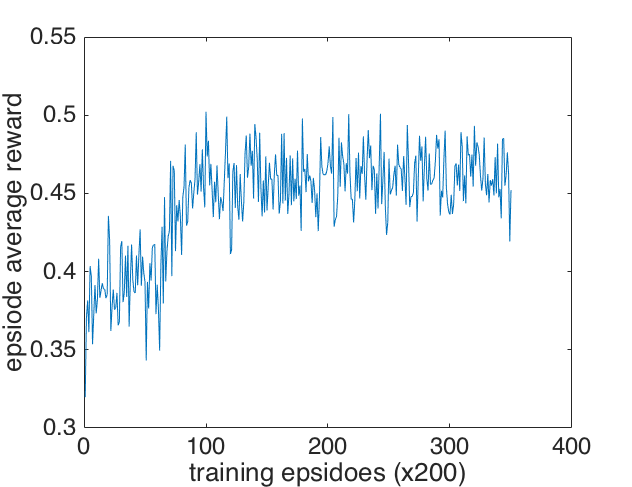
\includegraphics[width=\linewidth]{img/avg_r_iden5x5}
 	\caption{Average reward}
 	\label{fig:avg_r_iden5x5}
 \end{subfigure}
 ~
 \centering
 \begin{subfigure}[t]{0.49\textwidth}
 	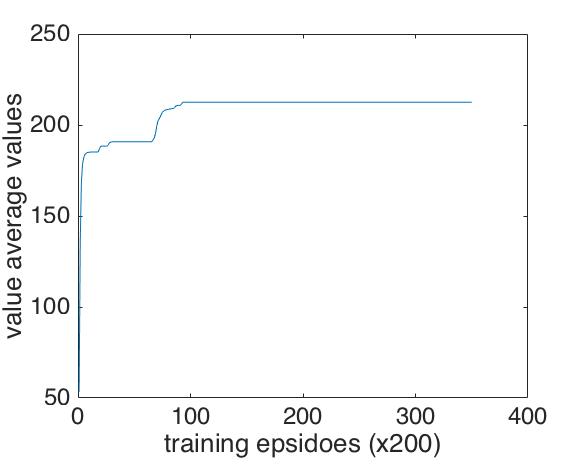
\includegraphics[width=\linewidth]{img/v_iden5x5}
 	\caption{Value function convergence}
 	\label{fig:v_iden5x5}
 \end{subfigure}
 \\
 \centering
 \begin{subfigure}[t]{0.49\textwidth}
 	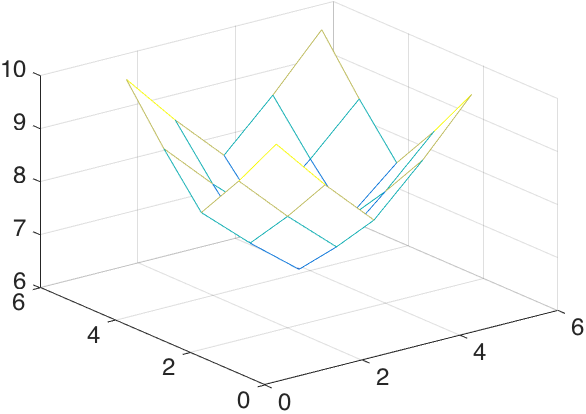
\includegraphics[width=\linewidth]{img/v3d_iden5x5}
 	\caption{Final value function on maze states}
 	\label{fig:v3d_iden5x5}
 \end{subfigure} 
 ~
 \centering
 \begin{subfigure}[t]{0.49\textwidth}
 	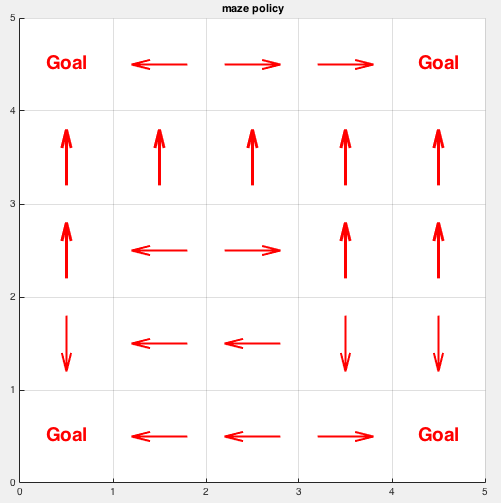
\includegraphics[width=\linewidth]{img/policy_iden5x5}
 	\caption{Final policy}
 	\label{fig:policy_iden5x5}
 \end{subfigure} 	
 \caption{5x5 maze. Identity Functions $f_{i}(s)=I(s=s_i)$ representation}
\end{figure}

Now let's compare above results with the exactly same task where Q functions was approximated by 25 basis identity state functions $f_{i}(s)=I(s=s_i)$
I have used the same learning parameters:
\begin{center}
	\begin{tabular}{| c | c | }
		\hline
		Learning rate $\eta$ &  0.2 \\ 
		\hline
		Exploration rate $\epsilon$ & 0.1 \\ 
		\hline
		Discount rate $\gamma$ & 0.9; \\
		\hline
	\end{tabular}
\end{center}

I have received the following convergence results:

\begin{center}
	\begin{tabular}{| c | c | }
		\hline
		Convergence criteria &  0.2 \\ 
		\hline
		Number of experiments & 10 \\ 
		\hline
	    Mean convergence time & 16220 $\pm$ 1475 episodes \\
		\hline
	\end{tabular}
\end{center}

Within its confidence intervals this results matches the convergence time obtained for tabular representation. 

When basic function approximation is applied the approximated value functions can be computed from weights $W(A,\ number\ of\ basis \ functions)$ and basis functions \\
$F(Sx, Sy,\ number\ of\ basis \ functions)$ using the following code snippet:

\begin{lstlisting}[language=Octave]
  % reshape(F, Sx * Sy, 25) % Sx*Sy x 25  
  % W' %  25 x A
  QQ = reshape(F, Sx * Sy, 25) * W'; % (Sx*Sy x 25) * (25 x A) = Sx*Sy x A
  VV = max(QQ,[],2); %Sx*Sy
  %approximated value function
  VV = reshape(VV, Sx, Sy);
\end{lstlisting}


Next, Figures \ref{fig:avg_r_iden5x5}, \ref{fig:v_iden5x5}, \ref{fig:v3d_iden5x5} are in good correspondence with its analogues from tabular representation on Figure \ref{fig:true5x5}. This is expected as when we are using 5x5 Identity functions for 5x5 maze the tabular representation and basis functions representation should be essentially the same. This can be seen by comparing the number of parameters to be learn. 
In tabular representation we learn the Q values $|Q(Sx, Sy, A)|=5*5*5=125$. In basis functions representation we learn weight matrix from Equation \ref{eq:simpleApprox} -> $|W(A,\ number\ of\ basis \ functions)| = 5*25=125$.
The final policy depicted on Figure \ref{fig:policy_iden5x5} differs from the one on Figure \ref{fig:policy_true5x5} but it is still optimal policy and the difference between them can be described by the fact that in this maze problem there are many equally optimal policies. 










%------------------ QUESTION 2 END ------------------------------











\section{Identity functions representation in 10x10 maze}
\begin{figure}[htbp!]
 \centering
 \begin{subfigure}[t]{0.49\textwidth}
 	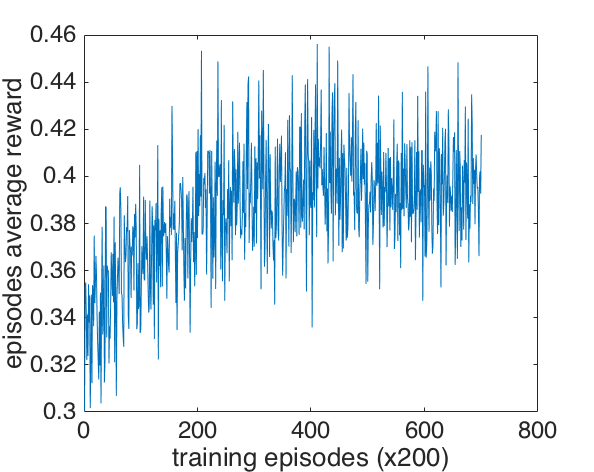
\includegraphics[width=\linewidth]{img/avg_r_true10x10}
 	\caption{Average reward}
 	\label{fig:avg_r_true10x10}
 \end{subfigure}
 ~
 \centering
 \begin{subfigure}[t]{0.49\textwidth}
 	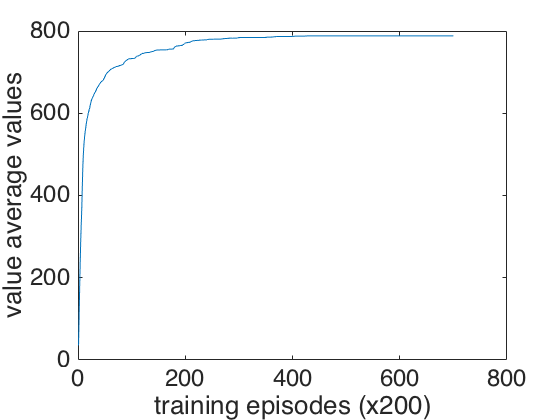
\includegraphics[width=\linewidth]{img/v_true10x10}
 	\caption{Value function convergence}
 	\label{fig:v_true10x10}
 \end{subfigure}
 \\
 \centering
 \begin{subfigure}[t]{0.49\textwidth}
 	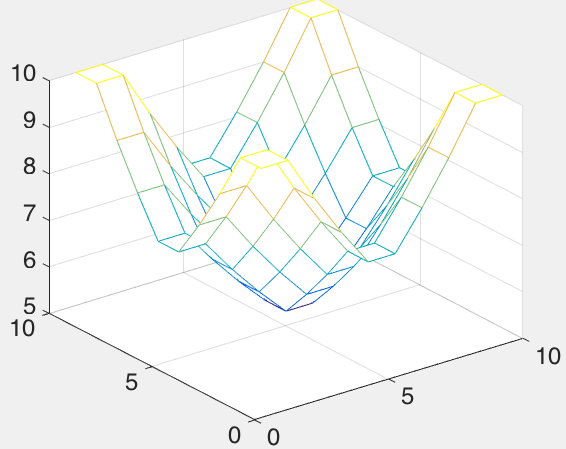
\includegraphics[width=\linewidth]{img/v3d_true10x10}
 	\caption{Final value function on maze states}
 	\label{fig:v3d_true10x10}
 \end{subfigure} 
 ~
 \centering
 \begin{subfigure}[t]{0.49\textwidth}
 	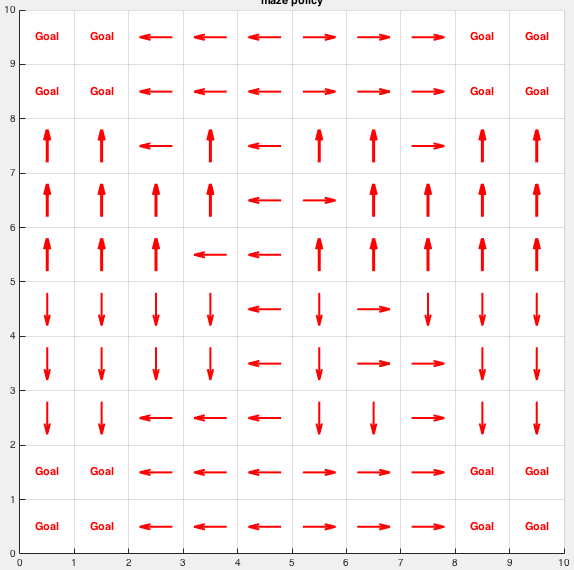
\includegraphics[width=\linewidth]{img/policy_true10x10}
 	\caption{Final policy}
 	\label{fig:policy_true10x10}
 \end{subfigure} 	
 \caption{10x10 maze. Table representation}
 \label{fig:true5x5}
\end{figure}

In this question identity basis functions evenly cover patches 2x2 of maze cells. It has been already shown how state identity functions are computed in that case in the first code listing of question 1.

Here, I redefine goals as patches 2x2 placed in the corners of the maze because in this representation agent doesn't have enough information to reach final goal reliably once it is within goal patch 2x2. It happens because for all closest neighbours around goal states the same identity functions will be activated.

First, we compute true results in tabular representation of Q function for maze 10x10. For that I have used the same learning parameters as in previous question:

\begin{center}
	\begin{tabular}{| c | c | }
		\hline
		Learning rate $\eta$ &  0.2 \\ 
		\hline
		Exploration rate $\epsilon$ & 0.1 \\ 
		\hline
		Discount rate $\gamma$ & 0.9; \\
		\hline
	\end{tabular}
\end{center}

On Figure \ref{fig:avg_r_true10x10} the average reward per episode has almost the same mean as on Figure \ref{fig:avg_r_true5x5} but it has significantly bigger variance in results. This can be described by the fact that now the maze has become bigger and average path to nearest the goal has become longer. However, the chances of appearing on the goal cell from the beginning has remained the same as $$



\section{Appendix}
Main launch code where simulation starts and all learning parameters
such as $\alpha$ (note that in the code I use eta instead for shortness), $\gamma$ and $\epsilon$ are specified:
%\lstinputlisting{code/rl_taxi_sim.m}

Defining supporting global variable which are the same for all simulations, such drop off locations, walls positions, etc. (except probably  - sometimes I change it):


%SARSA code:
%\lstinputlisting[language=Octave]{code/SARSA_episode.m}

\printbibliography[
    heading=bibintoc,
    title={References}
    ] %Prints the entire bibliography
    
    \clearpage

\end{document}